\documentclass[12pt]{article}
% REVISION NOTES %%%%%%%%%%%%%%%%%%%%%%%%%%%%%%%%%%%%%%%%%%%%
% 2008-0814 Location, Date, Time
% 2008-0814 fixed citations -- added bibliography.
%
%
\usepackage{geometry}                
\geometry{letterpaper}                   
%\geometry{landscape}                
\usepackage[parfill]{parskip}    
\usepackage{daves,fancyhdr,natbib,graphicx,dcolumn,amsmath,lastpage,url}
\usepackage{amsmath,amssymb,epstopdf,longtable}
\usepackage[final]{pdfpages}
\DeclareGraphicsRule{.tif}{png}{.png}{`convert #1 `dirname #1`/`basename #1 .tif`.png}
\pagestyle{fancy}
\lhead{CE 3305 -- Fluid Mechanics -- SPRING 2024}
\rhead{Name:\_\_\_\_\_\_\_\_\_\_\_\_\_\_\_\_\_\_\_\_\_\_\_\_\_\_\_\_\_\_\_\_\_\_\_\_\_\_\_\_\_\_\_\_}
\lfoot{CE 3305 -- Cleveland}
\cfoot{Page \thepage\ of \pageref{LastPage}}
\rfoot{REVISED: ~4 FEB 2024}
\renewcommand\headrulewidth{0pt}
%%%%%%%%%%%%%%%%%%%%%%%%%%%%%%%%%%%%%%%%%%%%%%%%%%%%%%%
\begin{document}
\section*{\center{ { CE 3305 -- Fluid Mechanics} {Exam 2} } }
\section*{Purpose}
Demonstrate ability to apply fluid mechanics and \textbf{problem solving principles} covering topics such as: Conservation of mass, continunity, conservation of linear momentum, and conservation of energy (modified bernoulli).
\section*{Instructions}
\begin{enumerate}
\item Put your name on each sheet you submit.  
\item Use additional sheets as needed. 
\item Begin each problem on a separate page.  Ok to disassemble to keep pages in order.
\item Do not write on the back of sheets (I won't look)
\item Use the \textbf{problem solving protocol} in the class notes.  The discussion section can simply be the word ``discussion'' 
\item Label and/or underline answers, be sure to include units.
\end{enumerate}
\section*{Allowed Resources}
\begin{enumerate}
\item Your notes
\item Your textbook
\item The mighty Internet with following proviso
\item  \textbf{You may not communicate with other people during the exam}
\end{enumerate}
\noindent\rule{\linewidth}{0.4pt}
\clearpage

\begin{enumerate}
\item The pipe below transports 200 kg/s of water. The pipe tees into a 5-cm-diameter pipe and a
7-cm-diameter pipe. The average velocity in the smaller-diameter pipe (5-cm-diameter pipe) is 25 m/s,

\begin{figure}[htbp] %  figure placement: here, top, bottom, or page
   \centering
   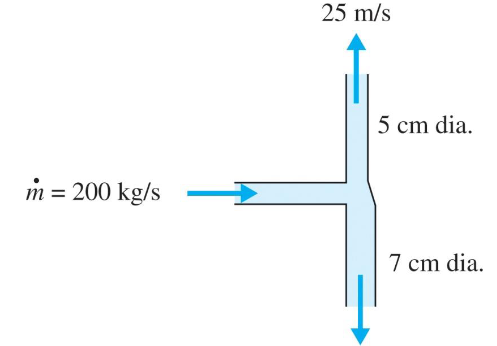
\includegraphics[width=4in]{continunity.png} 
   \caption{}
   \label{fig:continunity}
\end{figure}

Determine:
\begin{enumerate}
\item The flow rate in the larger pipe (7-cm-diameter pipe).
\end{enumerate}
\noindent\rule{\linewidth}{0.4pt}
\clearpage
%~\newline
%\clearpage
%\item A fixed mass of water has a bulk modulus of compressibility of $2.2 \times 10^{9} ~Pa$. \\ \\
%Determine:
%\begin{enumerate}
%\item The pressure increase ($\Delta p$) required to reduce the volume of a mass of water by 2-percent (2 \%)
%\end{enumerate}
%\noindent\rule{\linewidth}{0.4pt}
%\clearpage
%\noindent\rule{\linewidth}{0.4pt}
\item A vertical pipe with a smooth-transition reducer is monitored by a mercury manometer system as shown.

\begin{figure}[htbp] %  figure placement: here, top, bottom, or page
   \centering
   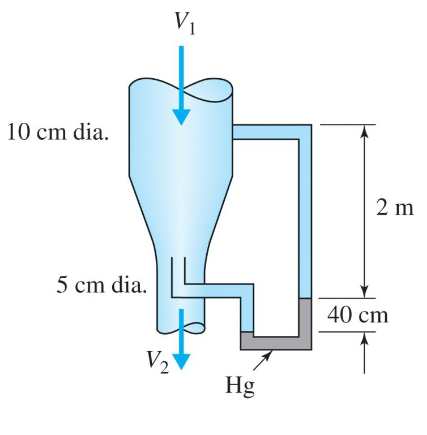
\includegraphics[width=4in]{venturiflow.png} 
   \caption{}
   \label{fig:venturiflow}
\end{figure}

Determine:
\begin{enumerate}
\item The approach velocity $V_1$ of the water in the vertical pipe; Assume negligible head losses (smooth-transition)
\end{enumerate}
\noindent\rule{\linewidth}{0.4pt}
%\clearpage
%~\newline
%\item A small spherical drop of water with diameter $d=4~mm$  and surface tension ($\sigma = 72.8 \times 10^{-3} \frac{N}{m}$) is depicted in the drawing below.

%\begin{figure}[h!] %  figure placement: here, top, bottom, or page
%   \centering
%   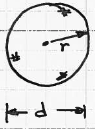
\includegraphics[width=1in]{drop.png} 
%   \caption{}
%   \label{fig:drop}
%\end{figure}

%Determine:
%\begin{enumerate}
%\item The gage pressure of the water in the drop.
%\end{enumerate}
%\noindent\rule{\linewidth}{0.4pt}
\clearpage
%\noindent\rule{\linewidth}{0.4pt}
\item A pipe discharges to the atmosphere just downstream of a plug as shown below.

\begin{figure}[h!] %  figure placement: here, top, bottom, or page
   \centering
   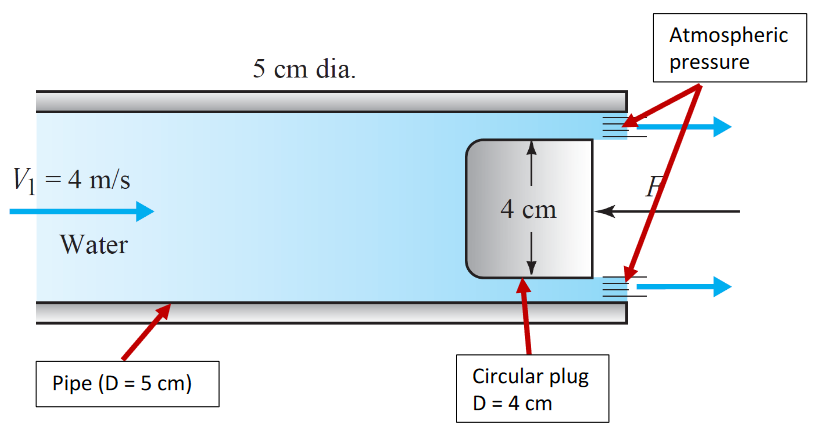
\includegraphics[width=4in]{plug-valve.png} 
   \caption{}
   \label{fig:plugvalve}
\end{figure}

Determine:
\begin{enumerate}
\item The force ,$F$, needed to hold the circular plug in the pipe as shown. Assume uniform velocity profiles;  Neglect viscous effects. 
\end{enumerate}
\noindent\rule{\linewidth}{0.4pt}
%\clearpage
%~\newline
\end{enumerate}
%%%%%%%%%%%%%%%%%%%%%%%%%%%%%%%%%%%%%%%%%%%%%%%%%%%%%%%%%%%%%%%%%%%%%%%%%%%%%%%%%%%%
\bibliographystyle{chicago}	         % (uses file "chicago.bst")
\end{document}


